\documentclass[12pt,a4paper]{report}
\usepackage[utf8]{inputenc}
\usepackage[inner=3.5cm,outer=2.5cm,bottom=3cm,top=2.5cm,pdftex]{geometry}
\usepackage{setspace}
\usepackage{graphicx}
\usepackage{rotating}
\usepackage[page]{appendix}
\usepackage{float}
\usepackage[font=small,labelfont=bf]{caption}
\usepackage{subfigure}
\usepackage{titlesec}
\usepackage[hidelinks]{hyperref}
\usepackage{listings}
\usepackage{textcomp}
\usepackage{fancyhdr}
\usepackage{multirow}
\usepackage{verbatim}	%makes it possible to comment out a section of text by using \begin{comment}...\end{comment}
\usepackage[table,xcdraw]{xcolor}
\usepackage{pifont}
\usepackage{mathptmx}
\usepackage{wrapfig}
\usepackage{ragged2e}
\usepackage[nottoc,notlot,notlof]{tocbibind}
\usepackage[norsk]{babel}

\definecolor{rockwoolcolor}{RGB}{155,0,0}

% Style chapter headings for preface and toc.
\setlength{\headheight}{15pt}
\titlespacing*{\chapter}{0pt}{0pt}{4ex}
\titleformat{\chapter}[display]
 {\bfseries\Large}
 {}
 {0pt}
 {\color{rockwoolcolor}\titlerule[2.0pt]\vspace{2ex}\filright\color{black}}
 [\color{rockwoolcolor}\vspace{2ex}{\titlerule[2.0pt]}]


\setstretch{1.25}
\begin{document}
\begin{titlepage}

\newcommand{\HRule}{\color{rockwoolcolor}\rule{\linewidth}{0.75mm}\color{black}} % Defines a new command for the horizontal lines, change thickness here

\center % Center everything on the page
 
%----------------------------------------------------------------------------------------
%	HEADING SECTIONS
%----------------------------------------------------------------------------------------
\ \\[1.5cm]
\textsc{\LARGE BI Handelshøyskolen}\\[1.5cm] % Name of your university/college
\textsc{\Large BTH 95031 Økonomistyring og investeringsanalyse}\\[2.5cm] % Major heading such as course name


%----------------------------------------------------------------------------------------
%	TITLE SECTION
%----------------------------------------------------------------------------------------

\HRule \\[0.4cm]
{ \huge \bfseries Investeringsanalyse for \\[0.5cm] ROCKWOOL International}\\[0.4cm] % Title of your document
\HRule \\[2.5cm]
 
%----------------------------------------------------------------------------------------
%	DATE & PLACE SECTION
%----------------------------------------------------------------------------------------

{\large \textbf{Innleveringsdato:}\\  \today}\\[1cm] % Date, change the \today to a set date if you want to be precise
{\large \textbf{Studiested:}\\  BI Nydalen}\\[3cm] % Date, change the \today to a set date if you want to be precise
 
%----------------------------------------------------------------------------------------

\textit{Denne oppgaven er gjennomført som en del av studiet ved Handelshøyskolen BI. Dette innebærer
ikke at Handelshøyskolen BI går god for de metoder som er anvendt, de resultater som er
fremkommet, eller de konklusjoner som er trukket.}
\vfill % Fill the rest of the page with whitespace

\end{titlepage}
{\RaggedRight
\pagestyle{fancy}

% empty default settings for fancy layout
\fancyhf{}

% table mark commands
\newcommand{\cmark}{\textcolor{green!80!black}{\ding{51}}}
\newcommand{\xmark}{\textcolor{red}{\ding{55}}}
\newcommand{\plusmark}{\textcolor{green!80!black}{\textbf{+}}}
\newcommand{\minusmark}{\textcolor{red}{\textbf{-}}}

% chapter, section, header and footer layout
\renewcommand{\sectionmark}[1]{\markright{\thesection ~ \ #1}}
\renewcommand{\chaptermark}[1]{\markboth{ #1}{}}
\renewcommand{\headrulewidth}{0.5pt}
\renewcommand{\footrulewidth}{0.5pt}

%head setting
%\fancyhead[L]{\textcolor{black} {\rightmark}}
\fancyfoot[C]{\textcolor{black} {\thepage}}

% Redefine the plain page style - used when the page is a chapter
\fancypagestyle{plain}{%
  \fancyhf{}%
  \renewcommand{\headrulewidth}{0pt}% Line at the header invisible
  \renewcommand{\footrulewidth}{0.5pt}% Line at the footer visible
  \fancyfoot[C]{\textcolor{black} {\thepage}}
}

% Avoid hyphenating
\tolerance=10
\emergencystretch=\maxdimen
\hyphenpenalty=10000
\hbadness=10000

\pagenumbering{roman}
\chapter*{Forord}



\chapter*{Sammendrag}
I desember 2018 besluttet ROCKWOOL International å investere i en ny elektrisk smelteovn på fabrikken i Moss. Konsernet produserer isolasjonsprodukter som utvinnes av vulkansk stein, og er verdens ledende leverandør av produkter og løsninger basert på steinull. Formålet med oppgaven er å utføre en investeringsanalyse på vegne av selskapet for å undersøke om prosjektet er lønnsomt. 

\indent \newline
For å vurdere lønnsomheten av prosjektet benytter vi oss av netto nåverdimetoden. Beregningen er basert på en differansekontantstrøm som er utarbeidet ved å sammenligne nåværende smelteteknologi med den nye elektriske smelteovnen. Kontantstrømmene neddiskonteres med relevant avkastningskrav justert for valutarisiko og business risk. Avkastningskravet er estimert gjennom beregning av selskapets egenkapitalbeta som brukes til å beregne egenkapitalkrav og selskapets totalkapitalkrav.

\indent \newline
I oppgaven drøfter vi ulike makroforhold som legges til grunn for fremtidig utvikling i isolasjonsbransjen. Den viktigste faktoren er det globale fokuset mot en grønnere fremtid. Analysen viser til flere usikkerhetsmomenter som er vanskelig å forutse hvordan vil utvikle seg i fremtiden. Sensitivitetsanalyser er derfor benyttet for å belyse hvordan endringer i forutsetningene vil påvirke netto nåverdi. I tillegg har vi utført en \textit{best-} og \textit{worst} case analyse for å gjøre ledelsen i selskapet bevisst på utfallsrommet investeringen befinner seg i.

\indent \newline
Differansekontantstrømmen  viser til en positiv netto nåverdi på 588,500 millioner kroner og gir støtte til å konkludere med at investeringen er lønnsom. I tillegg vil prosjektet styrke selskapets merkevare og gi bedre forutsetninger til å imøtekomme endringen i markedsutviklingen.


\setcounter{tocdepth}{2}
\tableofcontents
\addtocontents{toc}{~\hfill\textbf{Side}\par}
\listoffigures
\listoftables

% ----------- CHAPTERS ----------------

% Parts
\cleardoublepage
% Style chapter headings.
\titleformat{\chapter}[display]
 {\bfseries\Large}
 {}
 {0pt}
 {\color{rockwoolcolor}\titlerule[2.0pt]\vspace{2ex}\filright\color{black} \thechapter . }
 [\color{rockwoolcolor}\vspace{2ex}{\titlerule[2.0pt]}]
\pagenumbering{arabic}
\setcounter{page}{1}
\chapter{Innledning}
\section{Formål}
I denne oppgaven skal vi gjennomføre en investeringsanalyse av AS ROCKWOOL sin beslutning om å investere i en ny elektriske smelteovn. Formålet er å se hvorvidt dette er et lønnsomt prosjekt fra eiernes perspektiv ved tidspunktet for beslutningen. Vi vil gjøre leseren oppmerksom på at oppgaven vil analysere investeringen på bakgrunn av AS ROCKWOOL som et selvstendig selskap? (få frem at vi ikke legger vekt på at bedriften er en del av et konsern, evt finner vi ut av det senere, kanskje det går an å inkludere konsernet i oppgaven?)

\section{Problemstilling}
Problemstillingen vi ønsker å besvare er utarbeidet i samarbeid med AS ROCKWOOL, og lyder som følger:

\indent \newline
\textit{\textbf{Var investeringen av elektrisk smelteovn lønnsom på beslutningstidspunktet?}}

\indent \newline
Lønnsomhetsvurderingen vil baseres på en flerperiodisk nåverdianalyse med et formål om å maksimere eiernes interesser. I dette tilfellet vil investeringen ikke kun vurderes ut i fra et finansielt perspektiv, men også fra ROCKWOOL-konsernets eiere, som ønsker å implementere en mer miljøvennlig profil. Vurderingen vil gjennomføres på følgende grunnlag:

\begin{itemize}
\item Vurdere investeringen isolert sett.
\item Nåverdianalyse av virksomhetens fremtidige kontantstrømmer ved beslutning om å investere i ny produksjonsteknologi.
\item Nåverdianalyse av virksomhetens fremtidige kontantstrømmer ved beslutning om å ikke investere i ny. produksjonsteknologi (fortsette som før).
\item Nåverdianalyse av virksomhetens fremtidige kontantstrømmer ved beslutning om å investere i alternativt “grønt” produksjonsutstyr (BAT-løsning/brun energi).
\end{itemize}

\indent \newline
I tillegg vil vi gjennom scenario(scenarie?)-analyse skissere tre forskjellige fremtider for investeringen (best, basis og worst), for å gjøre ledelsen mest mulig forberedt på fremtidige beslutninger relatert til virksomhetens strategi. (kanskje legge til noe om støtte fra Enova også?) kan være at dette punktet skal smelles inn et annet sted også!

\chapter{ROCKWOOL International og byggisolasjonsbransjen}
Kapittelet vil gi en kort presentasjon av konsernet og datterselskapet AS ROCKWOOL. Videre vil det redegjøres for nåsituasjonen til Rockwool, og hvilke utfordringer virksomheten står overfor i dag.

\section{Om selskapet}
ROCKWOOL International er verdens største steinullprodusent med over 11.000 ansatte fordelt på salgskontorer og fabrikker i 39 land. Virksomheten baseres på utvinning av vulkansk stein for å produsere produkter, systemer og løsninger innenfor byggisolasjon. Selskapet hadde i 2018 salgsinntekter på 26,149 milliarder kroner og et årsresultat på 2,064 milliarder kroner \cite{annualReport}.

\subsection{AS ROCKWOOL}
AS ROCKWOOL er et heleid norsk datterselskap av ROCKWOOL international. Virksomhetens visjon er \textit{“AS ROCKWOOL skal være ledende leverandør av isolasjon, der positivt bidrag til et bedre miljø og brannsikring skal være førende”}. Datterselskapet består av 240 ansatte fordelt på to fabrikker og et salgskontor. Disse er lokalisert i henholdsvis Moss, Trondheim og Oslo. I 2018 hadde de salgsinntekter på 919 millioner kroner og leverte et årsresultat på litt over 86 millioner kroner \cite{osloRegnskap}.

\indent \newline
Produksjonsprosessen foregår ved at vulkansk stein og koks blir tilsatt i den varme enden av maskinen og deretter utsatt for enormt høye temperaturer i en smelteovn. Videre blir det tilsatt bindemiddel hvor den glødende massen blir omgjort til ullfibre før massen spinnes til steinull.

\begin{figure}[H]
\centering
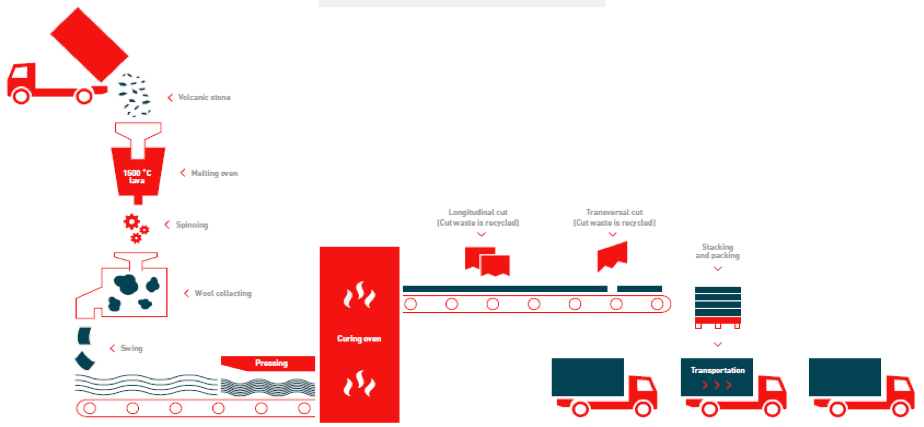
\includegraphics [scale=0.95]{bilder/produksjonsprosess.png}
\caption{Produksjonsprosess}
\label{fig:produksjonsprosess}
\end{figure}

\section{Historie}
I 1937 ble den første Rockwool-fabrikken etablert i Danmark. Få år senere utvidet konsernet med fabrikker i Larvik, Trondheim og Moss. Siden oppstarten i Norge har Rockwool basert virksomheten på utvinning av vulkansk stein, hvor produksjonsprosessen har forandret seg lite. Imidlertid investerte de nærmere en halv milliard kroner i nytt produksjonsutstyr på fabrikken i Moss i 2002, med et formål om å automatisere produksjonen. Dette har ført til mer enn en fordobling av produksjonskapasiteten. I løpet av de siste årene har de innført en lean-metode som de kaller for Ropex, med et ønske om å effektivisere virksomheten gjennom hele verdikjeden \cite{dagsavisen}.

\indent \newline
I 2016 vedtok Rockwool-konsernet å forplikte seg til FNs bærekraftsmål, hvorav 6 av 10 er implementert som interne konsernmål. Målene representerer forbedringer innenfor sikkerhet og helse, vannforbruk, energieffektivitet, avfallsresirkulering, og reduksjon i avfall og CO2-utslipp i produksjonsprosessen. Ett av målene er å redusere CO2-utslippet med 10\% innen 2022 og 20\% innen 2030.

\begin{figure}[H]
\centering
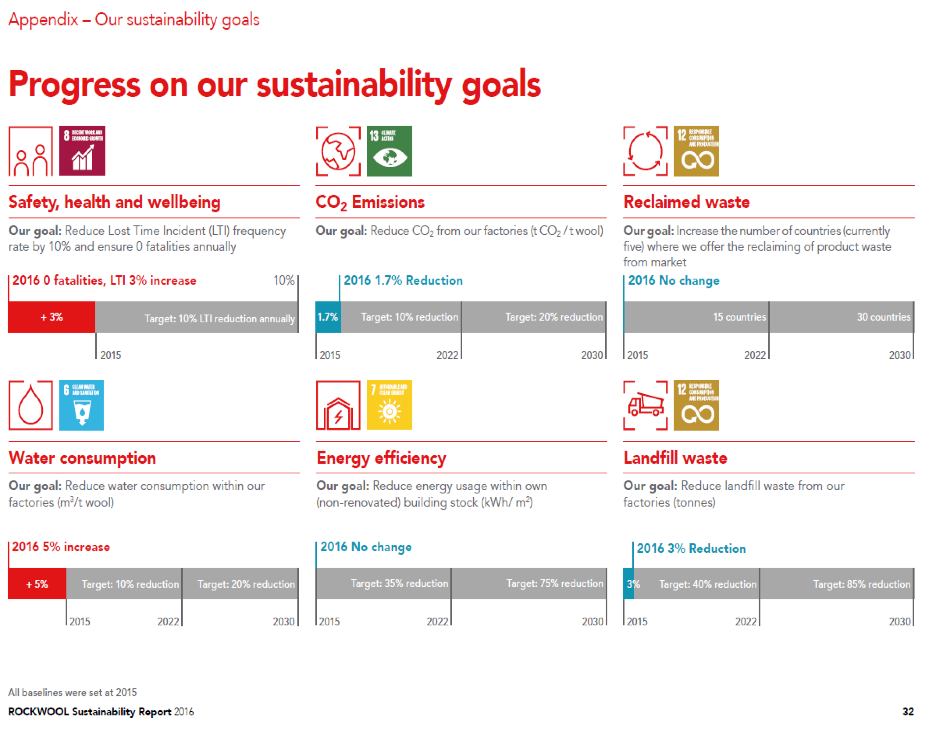
\includegraphics [scale=0.9]{bilder/baerkraftsmal.png}
\caption{Bærekraftsmål}
\label{fig:baerkraftsmal}
\end{figure}

\section{Markedet i Norge}  
Byggisolasjonsbransjen består av noen få store aktører som i likhet med Rockwool er datterselskaper av verdensomspennende konsern. Markedet karakteriseres av store mobilitetsbarrierer gjennom krav til kapitalintensive investeringer i spesialisert produksjonsutstyr. Rockwool har i flere år levert gode resultater, og er i dag markedets nest største aktør med en markedsandel på rundt 26\%. De mest nærliggende konkurrentene er Glava, Knauf, Sundolitt og Paroc, hvor Glava er markedets største med en markedsandel på 40\%. Kundene består i hovedsak av byggevarekjeder og entreprenører og sitter med høy forhandlingsmakt i form av at produsentene tilbyr lite differensierte produkter. Imidlertid leverer Rockwool og Paroc de mest differensierte produktene i form av produktegenskapene. De to virksomhetene er de eneste produsentene som leverer produkter som isolerer, er vannavstøtende, har lyddempende egenskaper og som er en god kilde til brannsikring. 

\indent \newline
Markedsveksten ligger på rundt 2\% og forventes å ligge på samme nivå i årene fremover. Dette viser til et modent marked. Den siste tiden har imidlertid Rockwool opplevd en lavere prosentvis vekst, grunnet en utvikling i markedet hvor miljøet blir vektlagt mer enn tidligere. Det blir vanligere for entreprenørene å BREEAM-sertifisere prosjektene sine. BREEAM er et miljøsertifiseringsverktøy for bygninger som legger vekt på miljøpåvirkning innenfor emner som energibruk, transport, materialer, avfall og forurensning\cite{breeam}. Dette påvirker spesielt produksjonsprosessen til isolasjonsprodusentene ved å stille krav til lavere utslipp. Rockwool sin nåværende smelteteknologi gir et høyere utslipp enn flere av konkurrentene, og er dermed en svakhet for virksomheten i forhold til å bli en foretrukken leverandør. 

\indent \newline
Det finnes også et annet økonomisk insentiv for produsentene til å redusere CO2-utslippet. Gjennom EØS-avtalen er Norge en del av Det europeiske kvotesystemet. Produsentene blir tildelt et visst antall kvoter og må kjøpe mer hvis utslippet overskrider det de får tildelt. Reduksjon i CO2-utslipp vil derfor resultere i lavere kostnader knyttet til drift.

\chapter{Beslutningsalternativer}
\section{El-ovn}
Rockwool besluttet i desember 2018 å investere i en ny smelteovn som vil benytte elektrisitet som energikilde. Beslutningen ble tatt etter å ha fått godkjent søknaden om 101,5 millioner kroner i støtte fra Enova. Enova er forvalter av Energifondet, og støtter norske bedrifter som ønsker en omstilling til lavutslippssamfunnet \cite{enova}. En elektrisk smelteovn er ikke tilgjengelig i markedet i dag, og investeringen krever at Rockwool selv utvikler nye og hensiktsmessige teknologiske løsninger tilpasset egen produksjon. Beregninger foretatt av selskapet viser til et investeringsbeløp på ca. 340 millioner kroner som fordeles i 2018, 2019 og 2020. Beløpet gjelder investeringer i innovasjon, teknologi og personalopplæring. 

\indent \newline
En el-ovn forventes å håndtere opp til 40\% gammel steinull (resirkulering), med en kapasitet på rundt 11.000 tonn steinullavfall fra byggeplasser. Dette tilsvarer mer enn totalt deponi av steinull per år fra byggmarkedet. Norge er i en særstilling når det gjelder avfall, hvor avfall til deponi, både fra produksjon og byggeplass, har vært relativt billig i flere år. Situasjonen er imidlertid i ferd med å endre seg da nye markeds- og myndighetskrav forventes fremover. Avfallet fra produksjonen representerer stangmøllemel (granulert ull) og små mengder avfall/kapp av ny isolasjon som returneres fra markedet. Øvrig produksjonsavfall består av ovnsbunn (jern, slagger og fines) og flyveaske. Teknologien vil kunne føre til en avfallsreduksjon på 19.677 tonn per år. Det tilsvarer en reduksjon på ca. 95\% sammenlignet med 2017.

\begin{table}[H]
  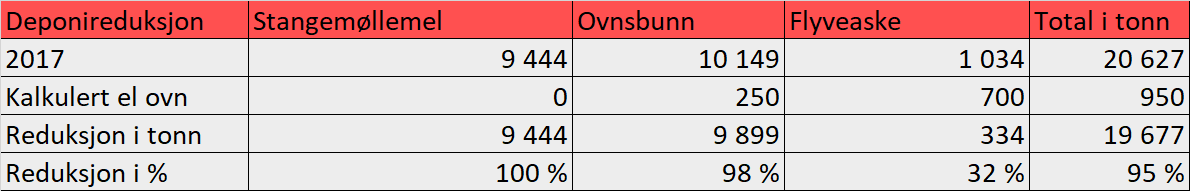
\includegraphics[width=\linewidth]{tabeller/deponireduksjon.png}
  \caption{Deponireduksjon}
  \label{tbl:deponireduksjon}
\end{table}

\indent \newline
Konvertering fra koks til elektrisitet vil også føre til store endringer med tanke på CO2-utslippet. Analyser fra Rockwool viser til en potensiell reduksjon i CO2-nivå med omtrent 80\%. Investeringen vil dermed føre til reduserte kostnader i forbindelse med CO2-kvoter, deponi og resirkulering. 

\begin{table}[H]
  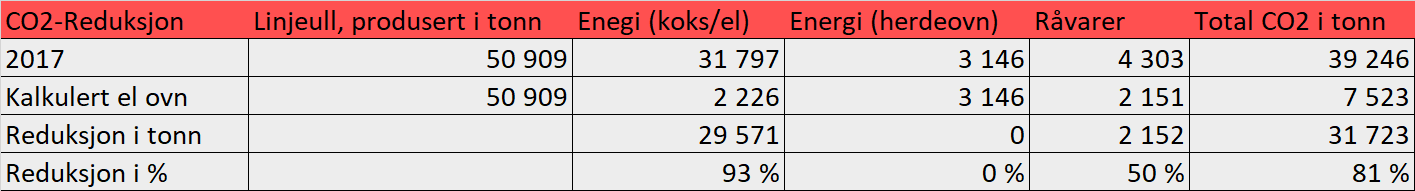
\includegraphics[width=\linewidth]{tabeller/co2reduksjon.png}
  \caption{CO2-reduksjon}
  \label{tbl:co2reduksjon}
\end{table}

\indent \newline
Investeringen baserer seg på utvikling innenfor teknologi og innovasjon i fire hovedelementer;

\begin{itemize}
\item[1.] Sikkerhet - Bygge den hittil største Submerged Arc Furnace (SAF) med lite smelteblad. En normal SAF-ovn med ønsket charge rate på 11,5 tonn per time vil ha en diameter på 8-9 meter og holde 189 tonn smelte. For å redusere risiko skal denne reduseres ned til 5,5-6 meter og holde 73 tonn smelte. Dette innebærer at en ny ovnstype med høyere “loadfaktor” må utvikles, noe som gir en høyere termisk belastning på ovnen og oppmuringsmaterialer.

\item[2.] Utvikle en SAF som kan håndtere en høy last samtidig med høy resirkuleringsandel. Dagens el-ovner har en begrensning i load og resirkuleringsfaktor, det vil si enten en høy load og lav resirkulering eller lav load og høy resirkulering. En resirkuleringsandel på 40\% vil stille nye krav til røykgassrensning. Resirkulert steinull inneholder mer organisk materiale sammenlignet med kun bruk av stein som råvare. Mengden rørgasser forventes derfor å øke sammenlignet med dagens produksjon.

\item[3.] Temperaturstabilitet - Utvikle en ny homogeniseringskanal.Fra ovn til spinnemaskiner er det over tre meter. Det ligger utfordringer i å sikre en stabil smeltetemperatur til spinnemaskinene. Det må derfor utvikles en homogeniseringskanal mellom ovn og eksisterende spinnere, da en slik kanal ikke er tilgjengelig i dag. Ved å sikre en stabil temperatur på +/- 10 grader celcius vil kanalen resultere i et høyere spinneutbytte.

\item[4.] Utvikle rett sammensetning av lining og effektivisere liningsbyttet. En høy grad av resirkulering vil stille nye krav til isolasjonsmateriale på innsiden av ovnen (lining). En ingeniørgruppe i Rockwool arbeider med å utvikle den rette sammensetningen for riktig lining. Erfaring viser at resirkulering øker slitasjen på liningen. Dette vil påvirke vedlikeholdsintervallene ved å gå fra hvert tredje år til hvert andre år. Målet er å redusere tiden det tar å skifte lining fra 3-4 uker til under 2 uker.
\end{itemize}

\indent \newline
I forbindelse med dimensjoneringen av smelteovnen vil selskapet produsere i et kapasitetsområde som ikke er prøvd ut tidligere. Overdimensjoneringen vil øke investeringen og risikoen i prosjektet, men anses som nødvendig for å opprettholde produksjonskapasiteten i Moss. Hvis temperaturstabillitet ikke oppnås, kan avfallsprosenten stige eksplosivt til 10-15\%. En marginal endring på 1\% resulterer i økte kostnader på 1,2 millioner kroner. Dette er isolert sett den største risikoen i prosjektet.

\indent \newline
I tillegg påløper det risiko knyttet til drift i form av en situasjon hvor det ikke oppnås full effekt. Dette fører til at resten av produksjonsanlegget ikke anvendes optimalt i forhold til produksjonsvolumene det er tilpasset til. Det vil også med stor sannsynlighet oppstå hyppigere og lengre stopp i produksjon, spesielt med tanke på liningslitasje. 

\section{Nåværende smelteteknologi}
Smelteteknologien som blir brukt i dag er en kupolovn, hvor energibærerne hovedsakelig består av koks og kalsinert karbon. Råvarer som benyttes er Anortositt, Gabbro, Fundia slagg, Dolomitt og Merox slagg. Per i dag har ikke kupolovnen nødvendig teknologi til å håndtere avfall fra byggeplasser.

\indent \newline
Å basere produksjonen hovedsakelig på fossile energibærere kan være risikofullt og kostbart, da markedsutviklingen går mot grønnere produkter. Klimarisikoen kommer til syne på et overordnet nivå, i form av Paris-avtalen og FNs bærekraftsmål, og på et underordnet nivå, i form av krav fra byggherrer og entreprenører. Rockwool har allerede erfart dette ved at byggaktørene har begynt å velge produkter som har et lavere CO2-avtrykk. Dette er gitt at øvrige byggetekniske krav er ivaretatt og prisen er konkurransedyktig. 

\indent \newline
Fokus på sirkulær økonomi har også fått større betydning de senere årene. Byggavfall er en stor kilde til avfall, og det forventes at markedet på sikt vil stille strengere krav til materialgjenvinning. I følge Erik Ølstad har eksempelvis Statsbygg signalisert at Rockwool må forberede seg på å endre dagens praksis og være i stand til å ta i mot retur av steinullavfall i fremtiden. 

\section{Brun smelteteknologi (BAT)}
En alternativ investering er en IMF-ovn (fluid bed ovn) hvor energibæreren er kull eller gass. Dette er en BAT-løsning (Best Available Technology) som kan bli gjennomført basert på Rockwool-konsernets egen smelteteknologi. Investeringen ligger på ca. 5 millioner kroner og innebærer redusert ovnsbunn og installasjon av full innvendig lining. Kostnaden for en slik smeltelinje ligger på samme nivå som en elektrisk smeltelinje. Imidlertid vil en BAT-oppdatering maksimalt resultere i 20-30\% CO2-reduksjon. Dette er derfor ikke en bærekraftig investering med en 10-års horisont. Høye vedlikeholdskostnader vil i tillegg gjøre det vanskelig for Rockwool å finansiere en slik løsning, da kapasiteten i Moss ikke er stor nok. I følge Rockwool var dette ikke et reelt alternativ, og beslutningen stod mellom å investere i el-teknologi eller å fortsette med nåværende teknologi. Vi vil på bakgrunn av dette ikke gå videre med å undersøke lønnsomheten av dette alternativet.


\chapter{Metode}
Metode omhandler aspekter knyttet til hvordan man går frem for å skaffe seg kunnskap. [Genaro Sucarrat; metode og økonometri].
\indent \newline
Metode er viktig i utredningen av økonomiske problemstillinger/analyser ettersom det spiller en sentral rolle i forberedelsene, gjennomføringen og tolkningen av undersøkelsene. I tillegg til å sikre god gjennomføring av egne analyser skal metodelæren bidra til å kunne evaluere styrker og svakheter ved andres undersøkelser. Metodelæren skilles i kvantitativ og kvalitativ metode. Kvantitativ metode tar sikte på å forklare eller anslå, mens kvalitativ metode tar sikte på å forstå.
Vi har benyttet oss av primær- og sekundærdata som er innhentet gjennom kvantitative og kvalitative metoder. Primærdata blir omtalt som data som blir hentet til et spesifikt formål, mens sekundærdata er data som allerede eksisterer og gjerne har tjent et annet formål tidligere.
 
\section{Kvantitativ metode}
For å utrede en netto nåverdianalyse har vi vært avhengig av historiske regnskapstall så vel som rent tekniske tall knyttet til produksjon og anslag rundt den nye smelteovnen. Rockwool har sendt oss en rekke dokumenter der vi har hentet ut relevante tall. Vi har brukt tallene for å modellere kontantstrømmer, avkastningskrav og sensitivitetsanalyser i Excel. Foruten innsikten fra Rockwool har vi brukt Proff-Forvalt, Norges Bank, NVE, samt flere relevante nettsider for å redegjøre for makroforhold og andre relevante beregninger.
 
\section{Kvalitativ metode}
Erik Ølstad, fabrikksjef i Moss, har vært vår kilde for innhenting av primærdata. Vi har ved flere anledninger møttes for uformelle samtaler der vi har fått belyst relevante spørsmål. Innsikten fra Erik har vært svært hjelpsom, både i form av kvantitative analyser, men han har også gitt oss en solid forståelse for markedet Rockwool opererer i.   
 
\indent \newline
Ref Genaro Sucarrat; [metode og økonometri- en moderne innføring 2. utgave]. Fagbokforlaget 2017.


\chapter{Teori}
\section{Netto nåverdimetoden}
Vi har i denne oppgaven valgt å besvare problemstillingen i lys av netto nåverdimetoden, da investeringen krever en flerperiodisk analyse (Espen Skaldehaug. forelesningsnotater/veiledningstime). Netto nåverdimetoden finner lønnsomheten til en investering ved å neddiskontere nåverdien av de fremtidige kontantstrømmene. Til tross for at NNV er den anbefalte metoden byr den på utfordringer. Estimering av fremtidige kontanstrømmer er i utgangspunktet umulig, men med fornuftige forutsetnigner og god markedsforståelse er det mulig å gjøre presise anslag. 

\indent \newline
\begin{math}
NNV={-X_0} + \frac {Xn}{1+r^n}
\end{math}

\indent \newline
Metoden belyser viktige momenter rundt tidshorisont og usikkerhet. Kroneverdien vil endres over tid, dette kan forklares med at man alternativt kunne plassert pengene der de vil forrente seg, inflasjon, og det faktum at det i prosjekter er knyttet usikkerhet til de fremtidige kontantstrømmene, og man vil ha kompensasjon for dette. Avkastningskravet vil hensynta denne usikkerheten. 

\indent \newline
En normal antakelse i forbindelse med bruk av netto nåverdimetoden er at man ønsker å maksimere eiernes profitt. Med bakgrunn i dette sier teorien at man alltid skal akseptere prosjekter med netto nåverdi > 0. I praksis vil dette bety en ekstraordinær avkastning på investert kapital. Dersom svaret blir positivt krever dette forklaring, gjerne gjennom effisiens-begrepet. 

\subsection*{Totalkapitalmetoden}
For å finne kontantstrømmen som skal tilkomme både eiere og långivere brukes totalkapitalmetoden. Metoden tar i bruk kontantstrømmen fra driften, finansielle poster utelukkes (Bøhren, Michalsen, Norli. S.351). Avkastningskravet skal reflektere avkastningen man alternativt kunne oppnådd ved å plassere midlene et annet sted med lik risiko (eStudie). WACC (Weighted average cost of capital) blir det relevante avkastningskravet ettersom modellen hensyntar investeringens finansiering gjennom en vekting av egenkapitalen og gjelden.

\[kT = kE * \frac{E}{E + G} + kG * (1-S) * \frac{G}{E + G}\]

\textit{hvor:
\begin{itemize}
    \item[] $kT$ = totalkapitalkostnaden etter skatt
    \item[] $kE$ = egenkapitalkostnaden etter skatt
    \item[] $kG$ = effektiv lånerente før skatt
    \item[] $s$ = relevant skattesats
    \item[] $E$ = egenkapitalens markedsverdi
    \item[] $G$ = gjeldens markedsverdi
\end{itemize}
}

\subsection*{Egenkapitalmetoden}
I egenkapitalmetoden er målet å finne kontantstrømmen til eierne. Sammenlignet med totalkapitalmetoden vil vi nå justere telleren for gjeldsopptak, renter og avdrag, inklusive renteskattefordelen (Bøgren, Michalsen, Norli. S.351). Kontantstrømmen vil så neddiskonteres med et avkastningskrav som reflekterer eiernes finansielle risiko. Det relevante avkastningskravet ved bruk av denne metoden er CAPM (Capital Asset Pricing Model).

\[kE = rf * (1-S) + \beta ek * [E(rm)-rf * (1-S)] \]

\textit{hvor:
\begin{itemize}
    \item[] $kE$ = egenkapitalkostnaden etter skatt
    \item[] $rf$ = risikofri rente
    \item[] $\beta ek$ = egenkapitalbeta
    \item[] $E(rm)$ = forventet avkastning på markedsporteføljen
    \item[] $s$ = skattesats
\end{itemize}
}
https://www.reuters.com/finance/stocks/overview/ROCKb.CO

\subsection{Estimering av risikofri rente \texorpdfstring{$(rf)$}{}}
Risikofri rente er avkastning en investor kan forvente å få uten å påta seg risiko. Et mål som ofte blir brukt på risikofri rente er statsobligasjoner. Den eneste måten man ikke skal kunne få denne avkastningen er hvis staten ikke klarer å betale sine forpliktelser. Rentenivået varier med løpetiden til statsobligasjonene, og det er derfor hensiktsmessig å velge rente på statsobligasjoner som er relevant for prosjektets levetid. Vi benytter derfor en effektiv rente på 10-års statsobligasjoner som risikofri rente. Per april 2019 var denne 1,71\%. https://www.norges-bank.no/tema/Statistikk/Rentestatistikk/Statsobligasjoner-Rente-Manedsgjennomsnitt-av-daglige-noteringer/

\subsection{Markedets risikopremie \texorpdfstring{$[E(rm) - rf *(1 - s)]$}{}}
Markedets risikopremie er den meravkastningen man krever ved å påta seg risiko. For å gjøre beregninger rundt dette er det nødvendig å se på de historiske dataene, da det ikke finnes noen god modell for å beregne fremtidige risikopremier. Fra 1976-2015 var den årlige norske risikopremien på 6,4\% (finansboka), men trenden de siste 20 årene har dog vært avtakende. PwC ferdigstilte i desember 2018 sitt mål for markedspremien, og denne lå på 5\%. Dette blir også vårt grunnlag for beregningen videre. 

https://www.pwc.no/no/publikasjoner/risikopremien-2018.html

\subsection{Estimering av betaverdi \texorpdfstring{($\beta ek$)}{}}
\[kE = rf * (1-S) + \beta ek * [E(rm)-rf * (1-S)] \]
\[0,0171 * 0,78 + 0,7 * (0,05 - 0,0171 * 0,78)= 3,9\%\]

\subsection{Blumes justeringsmodell}
Analyser gjennomført av Marshall Blume viser at selskapers BETA-verdier tenderer å bevege seg mot 1, og at selskaper med BETA-verdier nærme 1, er mer stabile enn de som er lengre unna. Blume mente derfor at det er hensiktsmessig å justere betaen ved følgende modell:

\[\beta justert = \beta raw * P +1,0 *(1-P)\]
Nyere forskning viser til at dette er fornuftig, derfor vil vi justere betaen for “mean reversion”. (forelesningsnotater “beregning av avkastningskrav” Pål Bertling-Hansen)

https://www.magma.no/hvordan-handtere-landrisiko-ved-investeringsbeslutninger1
https://www.infrontanalytics.com/fe-en/30064SD/Rockwool-International-A-S/Beta

\subsection{Beregning av egenkapitalens avkastningskrav (CAPM)}
\subsection{Totalkapitalens avkastningskrav}
\subsection{Internrentemetoden}
Internrentemetoden viser hvilket avkastningskrav som vil gi en avkastning på null i en netto nåverdiberegning. Metoden vil i vår oppgave kun bli brukt til å belyse hva som vil være høyeste mulig avkastningskrav for en lønnsom investering, da alle avkastningskrav høyere enn denne vil gi en negativ nåverdi.  

\subsection{Konsistensbetingelser}
En forutsetning for at netto nåverdimetoden skal forme et realistisk bilde av lønnsomheten i prosjektet er at konsistensbetingelsene legges til grunn. Med dette menes blant annet at man har frihet til å velge nominelle eller reelle tallstørrelser før eller etter skatt så lenge valgt metode er lik i teller og nevner. Vårt standpunkt tar utgangspunkt i de 5 grunnleggende konsistensbetingelsene (Forelesningsnotater).

\begin{itemize}
\item Nominelle tall - Tallene vi bruker vil være nominelle, altså vil inflasjon være hensyntatt. 
\item Etter skatt: Utregning av kontantstrøm og avkastningskrav vil bli beregnet etter fratrukket skatt ettersom skattereduksjonen aldri er lik i teller og nevner (forelesningsnotater).
\item Periodelengde: Teknisk levetid på investeringen vil antas å ha en levetid på 10 år, mens den økonomiske levetiden er antatt å være 20 år.
\item Kontantstrømmen: Bruke TK og eller EK ?
\item Risiko: Ettersom investeringen er av en ny teknologi som tidligere ikke er utprøvd foreligger det usikkerhet vedrørende investeringen. Usikkerheten knyttet til kontantstrømmene vil bli synliggjort i avkastningskravet. 
\end{itemize}

\subsection{Markedseffisiens}
Netto nåverdinalysen blir ikke tilstrekkelig uten å redegjøre for effisiensbegrepet. Et effisient marked betyr at all informasjon er priset inn i markedet. Dersom dette er sant vil det ikke være mulig å oppnå en ekstraordinær avkastning utover avkastningskravet. 
En NNV>0 betyr at investeringen har gitt en ekstraordinær avkastning.  

\subsection{Stikkord}
Effisient marked: Prisene reflekterer all relevant informasjon, NNV>0 er utenkelig, kontantstrømmen regnet for høy eller avkastningskravet for lavt, kombinasjon.
Ineffisient marked: AS ROCKWOOL vet noe de andre ikke vet (informasjonen varer ikke evig). Kan ha hef10 konkurransefortrinn. 






\chapter{Empiri (endre til makroforhold?)}
\section{Inflasjon}
Inflasjon er nødvendig å ta hensyn til ettersom pengeverdien i en flerperiodisk analyse vil forandre seg over tid. Å gi et korrekt anslag av hvordan dette vil utvikle seg i årene fremover er vanskelig på grunn av usikkerhet i markedet, men vi legger til grunn prognoser fra Norges Bank som anslår en fremtidig inflasjons økning på 2\%. Tolvmånedersendringen (Mars 2018- Mars 2019) ligger på 2,9\%, men er ventet å synke de kommende årene. (Andre oppgaver opererer med 2,5 prosent, vi kan eventuelt gjøre det). https://www.norges-bank.no/tema/Statistikk/Inflasjon/

% chapter heading as preface and toc
\titleformat{\chapter}[display]
 {\bfseries\Large}
 {}
 {0pt}
 {\color{rockwoolcolor}\titlerule[2.0pt]\vspace{2ex}\filright\color{black}}
 [\color{rockwoolcolor}\vspace{2ex}{\titlerule[2.0pt]}]
 
\renewcommand\bibname{Referanseliste}
\bibliographystyle{apalike}	% (uses file "plain.bst")
\bibliography{mineReferanser}		% expects file "mineReferanser.bib"
}

\end{document}
